\chapter{Binary Decision Diagrams}
\begin{figure}[h!]
\centering
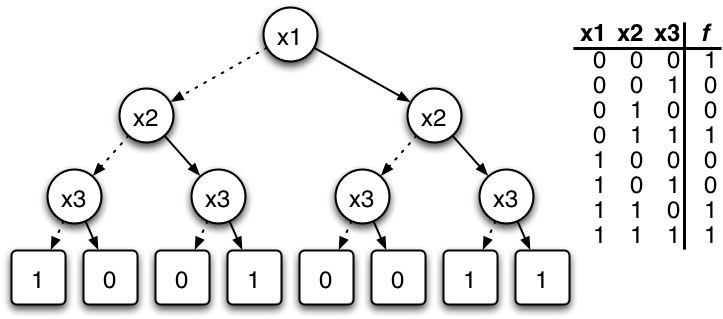
\includegraphics[width=4in]{binarydd/bdd-tree.png}
\caption{Binary decision tree and truth table 
for the function $
f(x_{1},
x_{2},x_{3})={\bar  {x}}_{1}{\bar 
 {x}}_{2}{\bar  {x}}_{3}+
x_{1}x_{2}+x_{2}x_{3} $ }
\label{fig-bdd-tree}
\end{figure}

\begin{figure}[h!]
\centering
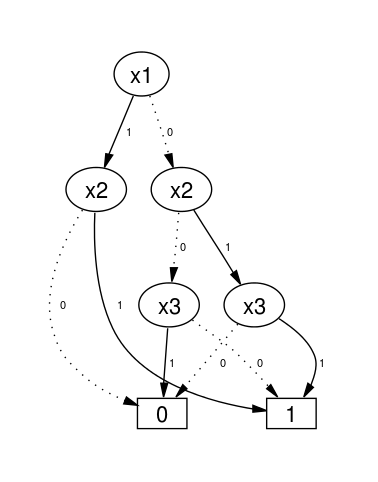
\includegraphics[width=2in]{binarydd/bdd.png}
\caption{BDD for the function $f$
of Fig.\ref{fig-bdd-tree}.} 
\label{fig-bdd}
\end{figure}

This chapter is based
on Wikipedia article Ref.\cite{wiki-bdd}.

Binary Decision Diagrams (BDDs)
can be understood as a special
case of Decision Trees (dtrees).
We will
assume
that the reader has read
Chapter \ref{ch-dtree} 
on dtrees before
tackling this chapter.

Both Figs.\ref{fig-bdd-tree}
and \ref{fig-bdd} were taken
from the aforementioned Wikipedia article. They
give a simple example of a function
$f:\bool^3\rarrow\bool$
represented in
Fig.\ref{fig-bdd-tree} as a
{\bf binary decision tree}
 and in Fig.\ref{fig-bdd} as a {\bf binary
decision diagram (BDD)}.
The goal 
of this chapter is
to represent both
figures as bnets with
almost the same graph structures.

We begin by noting
that the function
$f:\bool^3\rarrow\bool$
is a special case
of a probability
distribution
$P:\bool^3\rarrow[0,1]$.
In fact,
if we restrict $P$ to 
be deterministic, then
$P_{det}:\bool^3\rarrow\bool$
has the same domain
and range as $f$.
Henceforth,
we will refer to
$f(x_1,x_2,x_3)$
as $P(x_1,x_2,x_3)$,
keeping in mind that
we are restricting our
attention to deterministic
probability distributions. 

If we apply the chain
rule for conditional
probabilities to $P(x_1,x_2,x_3)$,
we get
\beq
P(x_1, x_2, x_3)=
P(x_3|x_1, x_2)P(x_2|x_1)P(x_1)
\;,
\eeq
which can be represented by the bnet:

\beq
\xymatrix{
\rvx_1\ar[d]\ar@/^1pc/[dd]\\
\rvx_2\ar[d]\\
\rvx_3
}
\label{eq-bdd-full-bnet}
\eeq
But
in Chapter \ref{ch-dtree},
we learned how
to represent
the bnet
of Eq.(\ref{eq-bdd-full-bnet})
as the bnet tree 
Eq.(\ref{eq-bdd-full-tree}).
In that tree,
the nodes
pose questions
with 3 possible answers $0,1,null$.


\beq
\xymatrix{
\ul{x_1?}\ar[d]\ar[dr]
\\
\ul{x_2|0?}\ar[d]\ar[dr]
&\ul{x_2|1?}\ar[dr]\ar[drr]
\\
\ul{x_3|00?}
&\ul{x_3|01?}
&\ul{x_3|10?}
&\ul{x_3|11?}
}
\label{eq-bdd-full-tree}
\eeq

The node transition probability
matrices, printed in blue,
for the bnet of Eq.(\ref{eq-bdd-full-tree})
are as follows.
If $x_1,x_2, x_3\in \{0,1,null\}$
and $a,b\in \bool$, then

\beq\color{blue}
P(\ul{x_1?}=x_1)=
\left\{
\begin{array}{ll}
P_{\rvx_1}(x_1)&\text{if $x_1\in \bool$}
\\
0&\text{if $x_1=null$}
\end{array}
\right.
\eeq


\beq\color{blue}
P(\ul{x_2|a?}=x_2\cond \ul{x_1?}=x_1)=
\left\{
\begin{array}{ll}
P_{\rvx_2|\rvx_1}(x_2|a)&\text{if $x_1=a$}
\\
\indi(x_2=null)&\text{otherwise}
\end{array}
\right.
\eeq

\beq\color{blue}
P(\ul{x_3|a,b?}=x_3\cond \ul{x_2|b?}=x_2)=
\left\{
\begin{array}{ll}
P_{\rvx_3|\rvx_1,\rvx_2}
(x_3|a,b)&\text{if $(x_1,x_2)=(a,b)$}
\\
\indi(x_3=null)&\text{otherwise}
\end{array}
\right.
\eeq
The bnet shown in
Eq.(\ref{eq-bdd-full-tree})
contains
the same info
and has 
the same graph structure
as the binary decision
tree Fig.\ref{fig-bdd-tree}.

The bnet shown in
Fig.\ref{fig-bdd}
appears to 
correspond to
the bnet of
Eq.(\ref{eq-bdd-bnet}).

\beq
\xymatrix{
\ul{x_1?}\ar[d]\ar[dr]
\\
\ul{x_2|0?}\ar[d]\ar[dr]
&\ul{x_2|1?}
\\
\ul{x_3|00?}
&\ul{x_3|01?}
&\bullet
&\bullet
}
\label{eq-bdd-bnet}
\eeq

\hrule
What happens
if we find out that
$P(x_3|x_1, x_2)=P(x_3|x_2)$ so that
one of the arcs of the
fully connected bnet Eq.(\ref{eq-bdd-full-bnet})
is unnecessary?
In that case,

\beq
P(x_1, x_2, x_3)=
P(x_3| x_2)P(x_2|x_1)P(x_1)
\;,
\eeq
which can be represented by the 
Markov chain bnet:

\beq
\xymatrix{
\rvx_1\ar[d]\\
\rvx_2\ar[d]\\
\rvx_3
}
\;.
\label{eq-bdd-markov}
\eeq

Following the prescriptions
of Chapter \ref{ch-dtree}, we
can represent
the bnet
of Eq.(\ref{eq-bdd-markov})
as the bnet tree 
Eq.(\ref{eq-bdd-markov-tree}).
In that tree,
the nodes
pose questions
with 3 possible answers $0,1,null$.

\beq
\xymatrix{
\ul{x_1?}\ar[d]\ar[dr]
\\
\ul{x_2|0?}\ar[d]\ar[dr]
&\ul{x_2|1?}\ar[dr]\ar[drr]
\\
\ul{x_3|\_,0?}
&\ul{x_3|\_,1?}
&\ul{x_3|\_,0?}
&\ul{x_3|\_,1?}
}
\label{eq-bdd-markov-tree}
\eeq



